\section{Results}


Forecasting bubbles from imidiately observable characteristics of the introducers of those coins to the forum appears to be a challenging task: of our baselines in terms of raw activity, number of members who responded and weather the code embodies substantial changes, none achieve out of sample error rates when tested in our methodology.

This is a challenging task, and models that rely on either simple activity or network metrics metrics show almost no predictive out-of-sample power, unable to explain even 1\% of the variation in either task,
our best models perform an order of magnitude better in both tasks.
%JULIAN: R^2 of 0.1 (if I interpret correctly) doesn't sound impressive until you've argued the fundamental difficulty of the problem, you might wait to mention such numbers.
%JULIAN: Would sound more impressive if you just said "it performs an order of magnitude better"
The main driver of our explanatory power is the centrality of a user in the directed network derived from the forum. 
This effect appears to be mediated by whether a coin involves a nontrivial technological change, the direction of the interaction reversing depending on whether it relates to magnitude or severity.
%JULIAN: Above sentence is tough to parse, but kind of an important one.
Both the severity and the magnitude of bubbles increases with the centrality of the user who introduces the coins in the forums.  
Interestingly this effect is concentrated in different ways depending on whether the coin software is more than a trivial modification: trivial coins have more severe bubbles the more central their introducers are, while volume is greater the more central the introducer of a nontrivial coin is.




\begin{figure}[h]
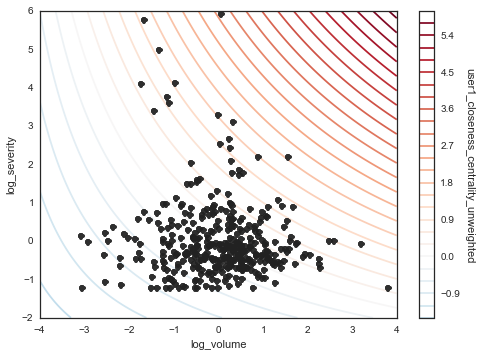
\includegraphics[width=\columnwidth]{centrality_volume_severity}
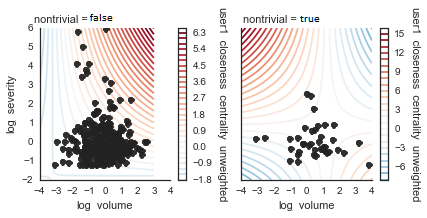
\includegraphics[width=\columnwidth]{centrality_volume_severity_nontrivial}
\end{figure}




\begin{figure}[h]
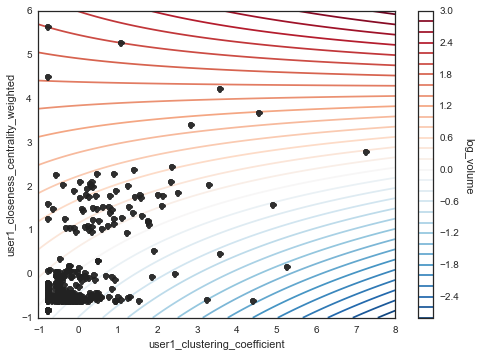
\includegraphics[width=\columnwidth]{cluster_closeness_volume}
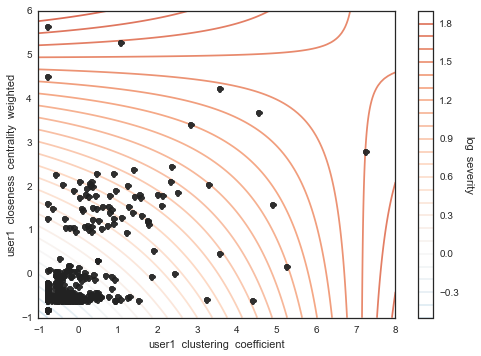
\includegraphics[width=\columnwidth]{cluster_closeness_severity}
\end{figure}

